% Options for packages loaded elsewhere
\PassOptionsToPackage{unicode}{hyperref}
\PassOptionsToPackage{hyphens}{url}
%
\documentclass[
  11pt,
  b5paper,
  nottoc]{book}

\usepackage{amsmath,amssymb}
\usepackage{iftex}
\ifPDFTeX
  \usepackage[T1]{fontenc}
  \usepackage[utf8]{inputenc}
  \usepackage{textcomp} % provide euro and other symbols
\else % if luatex or xetex
  \usepackage{unicode-math}
  \defaultfontfeatures{Scale=MatchLowercase}
  \defaultfontfeatures[\rmfamily]{Ligatures=TeX,Scale=1}
\fi
\usepackage{lmodern}
\ifPDFTeX\else  
    % xetex/luatex font selection
\fi
% Use upquote if available, for straight quotes in verbatim environments
\IfFileExists{upquote.sty}{\usepackage{upquote}}{}
\IfFileExists{microtype.sty}{% use microtype if available
  \usepackage[]{microtype}
  \UseMicrotypeSet[protrusion]{basicmath} % disable protrusion for tt fonts
}{}
\makeatletter
\@ifundefined{KOMAClassName}{% if non-KOMA class
  \IfFileExists{parskip.sty}{%
    \usepackage{parskip}
  }{% else
    \setlength{\parindent}{0pt}
    \setlength{\parskip}{6pt plus 2pt minus 1pt}}
}{% if KOMA class
  \KOMAoptions{parskip=half}}
\makeatother
\usepackage{xcolor}
\usepackage[left=2cm, right=2cm, top=2.5cm, bottom=2.5cm]{geometry}
\setlength{\emergencystretch}{3em} % prevent overfull lines
\setcounter{secnumdepth}{5}
% Make \paragraph and \subparagraph free-standing
\makeatletter
\ifx\paragraph\undefined\else
  \let\oldparagraph\paragraph
  \renewcommand{\paragraph}{
    \@ifstar
      \xxxParagraphStar
      \xxxParagraphNoStar
  }
  \newcommand{\xxxParagraphStar}[1]{\oldparagraph*{#1}\mbox{}}
  \newcommand{\xxxParagraphNoStar}[1]{\oldparagraph{#1}\mbox{}}
\fi
\ifx\subparagraph\undefined\else
  \let\oldsubparagraph\subparagraph
  \renewcommand{\subparagraph}{
    \@ifstar
      \xxxSubParagraphStar
      \xxxSubParagraphNoStar
  }
  \newcommand{\xxxSubParagraphStar}[1]{\oldsubparagraph*{#1}\mbox{}}
  \newcommand{\xxxSubParagraphNoStar}[1]{\oldsubparagraph{#1}\mbox{}}
\fi
\makeatother

\usepackage{color}
\usepackage{fancyvrb}
\newcommand{\VerbBar}{|}
\newcommand{\VERB}{\Verb[commandchars=\\\{\}]}
\DefineVerbatimEnvironment{Highlighting}{Verbatim}{commandchars=\\\{\}}
% Add ',fontsize=\small' for more characters per line
\usepackage{framed}
\definecolor{shadecolor}{RGB}{241,243,245}
\newenvironment{Shaded}{\begin{snugshade}}{\end{snugshade}}
\newcommand{\AlertTok}[1]{\textcolor[rgb]{0.68,0.00,0.00}{#1}}
\newcommand{\AnnotationTok}[1]{\textcolor[rgb]{0.37,0.37,0.37}{#1}}
\newcommand{\AttributeTok}[1]{\textcolor[rgb]{0.40,0.45,0.13}{#1}}
\newcommand{\BaseNTok}[1]{\textcolor[rgb]{0.68,0.00,0.00}{#1}}
\newcommand{\BuiltInTok}[1]{\textcolor[rgb]{0.00,0.23,0.31}{#1}}
\newcommand{\CharTok}[1]{\textcolor[rgb]{0.13,0.47,0.30}{#1}}
\newcommand{\CommentTok}[1]{\textcolor[rgb]{0.37,0.37,0.37}{#1}}
\newcommand{\CommentVarTok}[1]{\textcolor[rgb]{0.37,0.37,0.37}{\textit{#1}}}
\newcommand{\ConstantTok}[1]{\textcolor[rgb]{0.56,0.35,0.01}{#1}}
\newcommand{\ControlFlowTok}[1]{\textcolor[rgb]{0.00,0.23,0.31}{\textbf{#1}}}
\newcommand{\DataTypeTok}[1]{\textcolor[rgb]{0.68,0.00,0.00}{#1}}
\newcommand{\DecValTok}[1]{\textcolor[rgb]{0.68,0.00,0.00}{#1}}
\newcommand{\DocumentationTok}[1]{\textcolor[rgb]{0.37,0.37,0.37}{\textit{#1}}}
\newcommand{\ErrorTok}[1]{\textcolor[rgb]{0.68,0.00,0.00}{#1}}
\newcommand{\ExtensionTok}[1]{\textcolor[rgb]{0.00,0.23,0.31}{#1}}
\newcommand{\FloatTok}[1]{\textcolor[rgb]{0.68,0.00,0.00}{#1}}
\newcommand{\FunctionTok}[1]{\textcolor[rgb]{0.28,0.35,0.67}{#1}}
\newcommand{\ImportTok}[1]{\textcolor[rgb]{0.00,0.46,0.62}{#1}}
\newcommand{\InformationTok}[1]{\textcolor[rgb]{0.37,0.37,0.37}{#1}}
\newcommand{\KeywordTok}[1]{\textcolor[rgb]{0.00,0.23,0.31}{\textbf{#1}}}
\newcommand{\NormalTok}[1]{\textcolor[rgb]{0.00,0.23,0.31}{#1}}
\newcommand{\OperatorTok}[1]{\textcolor[rgb]{0.37,0.37,0.37}{#1}}
\newcommand{\OtherTok}[1]{\textcolor[rgb]{0.00,0.23,0.31}{#1}}
\newcommand{\PreprocessorTok}[1]{\textcolor[rgb]{0.68,0.00,0.00}{#1}}
\newcommand{\RegionMarkerTok}[1]{\textcolor[rgb]{0.00,0.23,0.31}{#1}}
\newcommand{\SpecialCharTok}[1]{\textcolor[rgb]{0.37,0.37,0.37}{#1}}
\newcommand{\SpecialStringTok}[1]{\textcolor[rgb]{0.13,0.47,0.30}{#1}}
\newcommand{\StringTok}[1]{\textcolor[rgb]{0.13,0.47,0.30}{#1}}
\newcommand{\VariableTok}[1]{\textcolor[rgb]{0.07,0.07,0.07}{#1}}
\newcommand{\VerbatimStringTok}[1]{\textcolor[rgb]{0.13,0.47,0.30}{#1}}
\newcommand{\WarningTok}[1]{\textcolor[rgb]{0.37,0.37,0.37}{\textit{#1}}}

\providecommand{\tightlist}{%
  \setlength{\itemsep}{0pt}\setlength{\parskip}{0pt}}\usepackage{longtable,booktabs,array}
\usepackage{calc} % for calculating minipage widths
% Correct order of tables after \paragraph or \subparagraph
\usepackage{etoolbox}
\makeatletter
\patchcmd\longtable{\par}{\if@noskipsec\mbox{}\fi\par}{}{}
\makeatother
% Allow footnotes in longtable head/foot
\IfFileExists{footnotehyper.sty}{\usepackage{footnotehyper}}{\usepackage{footnote}}
\makesavenoteenv{longtable}
\usepackage{graphicx}
\makeatletter
\def\maxwidth{\ifdim\Gin@nat@width>\linewidth\linewidth\else\Gin@nat@width\fi}
\def\maxheight{\ifdim\Gin@nat@height>\textheight\textheight\else\Gin@nat@height\fi}
\makeatother
% Scale images if necessary, so that they will not overflow the page
% margins by default, and it is still possible to overwrite the defaults
% using explicit options in \includegraphics[width, height, ...]{}
\setkeys{Gin}{width=\maxwidth,height=\maxheight,keepaspectratio}
% Set default figure placement to htbp
\makeatletter
\def\fps@figure{htbp}
\makeatother
% definitions for citeproc citations
\NewDocumentCommand\citeproctext{}{}
\NewDocumentCommand\citeproc{mm}{%
  \begingroup\def\citeproctext{#2}\cite{#1}\endgroup}
\makeatletter
 % allow citations to break across lines
 \let\@cite@ofmt\@firstofone
 % avoid brackets around text for \cite:
 \def\@biblabel#1{}
 \def\@cite#1#2{{#1\if@tempswa , #2\fi}}
\makeatother
\newlength{\cslhangindent}
\setlength{\cslhangindent}{1.5em}
\newlength{\csllabelwidth}
\setlength{\csllabelwidth}{3em}
\newenvironment{CSLReferences}[2] % #1 hanging-indent, #2 entry-spacing
 {\begin{list}{}{%
  \setlength{\itemindent}{0pt}
  \setlength{\leftmargin}{0pt}
  \setlength{\parsep}{0pt}
  % turn on hanging indent if param 1 is 1
  \ifodd #1
   \setlength{\leftmargin}{\cslhangindent}
   \setlength{\itemindent}{-1\cslhangindent}
  \fi
  % set entry spacing
  \setlength{\itemsep}{#2\baselineskip}}}
 {\end{list}}
\usepackage{calc}
\newcommand{\CSLBlock}[1]{\hfill\break\parbox[t]{\linewidth}{\strut\ignorespaces#1\strut}}
\newcommand{\CSLLeftMargin}[1]{\parbox[t]{\csllabelwidth}{\strut#1\strut}}
\newcommand{\CSLRightInline}[1]{\parbox[t]{\linewidth - \csllabelwidth}{\strut#1\strut}}
\newcommand{\CSLIndent}[1]{\hspace{\cslhangindent}#1}

\usepackage{booktabs}
\usepackage{multirow}
\usepackage{array,graphicx}
\usepackage{wrapfig}
\usepackage[normalem]{ulem}
\usepackage{lscape}
\usepackage{rotating}
\useunder{\uline}{\ul}{}
\usepackage{float}
\floatplacement{figure}{H}
\renewcommand{\chaptername}{Capitolul}
\renewcommand{\contentsname}{Cuprins}
\renewcommand\listfigurename{Lista figurilor}
\renewcommand\listtablename{Lista tabelelor}
\renewcommand\figurename{Figura}
\renewcommand\tablename{Tabel}
\renewcommand\bibname{Bibliografie}
\newcommand*\rot{\rotatebox{90}}
\usepackage{tocbibind}
\makeatletter
\@ifpackageloaded{bookmark}{}{\usepackage{bookmark}}
\makeatother
\makeatletter
\@ifpackageloaded{caption}{}{\usepackage{caption}}
\AtBeginDocument{%
\ifdefined\contentsname
  \renewcommand*\contentsname{Table of contents}
\else
  \newcommand\contentsname{Table of contents}
\fi
\ifdefined\listfigurename
  \renewcommand*\listfigurename{Lista figurilor}
\else
  \newcommand\listfigurename{Lista figurilor}
\fi
\ifdefined\listtablename
  \renewcommand*\listtablename{Lista tabelelor}
\else
  \newcommand\listtablename{Lista tabelelor}
\fi
\ifdefined\figurename
  \renewcommand*\figurename{Figura}
\else
  \newcommand\figurename{Figura}
\fi
\ifdefined\tablename
  \renewcommand*\tablename{Tabel}
\else
  \newcommand\tablename{Tabel}
\fi
}
\@ifpackageloaded{float}{}{\usepackage{float}}
\floatstyle{ruled}
\@ifundefined{c@chapter}{\newfloat{codelisting}{h}{lop}}{\newfloat{codelisting}{h}{lop}[chapter]}
\floatname{codelisting}{Listing}
\newcommand*\listoflistings{\listof{codelisting}{List of Listings}}
\makeatother
\makeatletter
\makeatother
\makeatletter
\@ifpackageloaded{caption}{}{\usepackage{caption}}
\@ifpackageloaded{subcaption}{}{\usepackage{subcaption}}
\makeatother

\ifLuaTeX
  \usepackage{selnolig}  % disable illegal ligatures
\fi
\usepackage{bookmark}

\IfFileExists{xurl.sty}{\usepackage{xurl}}{} % add URL line breaks if available
\urlstyle{same} % disable monospaced font for URLs
\hypersetup{
  pdftitle={Analiza datelor economico-sociale},
  pdfauthor={Ciprian Alexandru-Caragea},
  hidelinks,
  pdfcreator={LaTeX via pandoc}}


\title{Analiza datelor economico-sociale}
\usepackage{etoolbox}
\makeatletter
\providecommand{\subtitle}[1]{% add subtitle to \maketitle
  \apptocmd{\@title}{\par {\large #1 \par}}{}{}
}
\makeatother
\subtitle{cu aplicații și exemple în R, Python, Excel și PowerBI}
\author{Ciprian Alexandru-Caragea}
\date{2024-09-29}

\begin{document}
\frontmatter
\maketitle

\renewcommand*\contentsname{Cuprins}
{
\setcounter{tocdepth}{1}
\tableofcontents
}
\listoffigures
\listoftables

\mainmatter
\bookmarksetup{startatroot}

\chapter*{Despre autor}\label{despre-autor}
\addcontentsline{toc}{chapter}{Despre autor}

\markboth{Despre autor}{Despre autor}

\setcounter{page}{3}

\textbf{Ciprian Alexandru-Caragea} este conferenţiar universitar la
Facultatea de Management Financiar, Universitatea Ecologică din
București și Analist de Date la diverse instituții internaționale.\\

\begin{wrapfigure}{r}{0.3\textwidth}
  \begin{center}
    
\includegraphics[width=0.3\textwidth]{images/Ciprian_DGINS2018.jpg}
  \end{center}
\end{wrapfigure}

Titlul de doctor în Economie l-a obţinut sub egida Academiei Române,
Institutul de Economie Naţională.\\
A participat la un program de studii postdoctorale în care a implementat
utilizarea software-ului R ca instrument de analiză a evoluției
indicilor bursieri.\\
Activitatea sa didactică se concentrează, în principal, în domeniul
burselor de valori, prin cursuri și seminarii la programele de licență
și masterat (Piețe de capital, Managementul Portofoliului, Piețe
internaționale de capital).\\
A participat la diverse proiecte de cercetare, workshop-uri, conferințe
naționale și internaționale. Activitatea de cercetare a fost pusă în
valoare prin publicarea studiilor în reviste din țară și din Europa,
precum și în baze de date internaționale recunoscute (RePEC, DOAJ,
EBSCO).\\
În prezent, în cadrul Institului Național de Statistică, participă ca
expert în proiecte BigData și utilizează software-ul de analiză
statistică R pentru Data cleaning, Data Matching, Web Scraping, analize
de date și vizualizare, Data mining, Data integration, data processing,
data validation, dar și utilizarea datelor din sursele administrative
pentru realizarea de statistici oficiale.

\href{http://www.researcherid.com/rid/V-2168-2017}{ResearcherID:
V-2168-2017}\\
https://orcid.org/0000-0001-8215-6671

\bookmarksetup{startatroot}

\chapter*{Introducere}\label{introducere}
\addcontentsline{toc}{chapter}{Introducere}

\markboth{Introducere}{Introducere}

\begin{quote}
``\ldots acum nu mai e nimic nou de descoperit;\\
tot ce rămâne e doar măsurătoarea din ce în ce mai precisă''

--- Lord Kelvin (1894)
\end{quote}

Cartea tipărită merită răsfoită. Trăim în vremea în care internetul
facilitează comunicarea globală, informația fiind disponibilă oricând și
oricum. Toată lumea, de la oameni de știință și până la copii de vârstă
școlară primesc și oferă informații și propagă idei pe calea
internetului. Tirajele publicațiilor, cărților și manualelor tipărite
sunt în scădere în întreaga lume, în timp ce postările online captează
atenția omenirii.\\
Obiectivul principal al cărții pe care o propun este de a fi un ghid
cuprinzător, în termeni de concepte și tehnici, reprezentativ și, mai
ales, practic, în ceea ce privește utilizarea instrumentelor software de
analiză statistică, R fiind principalul software utilizat pentru
aplicațiile propuse. Ca abordare generală, cartea prezintă principalele
concepte utilizate în statistică, cu exemple și explicații descriptive.
Exemplele din viața economică - cele mai multe dintre ele bazate pe date
statistice reale - problemele rezolvate, dar și cele propuse, acoperă o
arie cuprinzătoare de tematici, cititorul având șansa de a fi introdus
în sfera aplicativă a conceptelor teoretice parcurse.\\
Cartea este destinată tuturor celor care doresc să înțeleagă, prin
mijloace științifice, fenomenele economice și sociale, sub aspectul
măsurării cantitative și din perspectiva determinării cauzale. Deși se
adresează, în principal, studenților care se pregătesc să devină
specialiști în științele economice, lucrarea este utilă și celor care
își propun să cunoască un domeniu atât de frumos și de captivant. Tocmai
nevoia de informații, din ce în ce mai complexe, dar și posibilitățile
de calcul avansat cu ajutorul soft-urilor tot mai performante, au condus
la crearea unui bazin imens de date care pot fi cu ușurință exploatate
pe baza analizei statistice. Poate că acesta este și motivul pentru care
statistica rămâne o disciplină percepută ca fiind adesea prea
matematizată, destinată specialiștilor. Pentru mulți cititori, mai ales
dintre cei care nu au o formare bazată pe un aparat matematic, studiul
fenomenelor economice prin metode statistice și matematice, presupune un
efort deosebit. Din acest motiv, am încercat să tratez aspectele
teoretice, dar și problemele cu aplicație practică din sfera economică,
într-o manieră simplă, accesibilă. Așadar, lucrarea are menirea de a
facilita înțelegerea conceptelor fundamentale cu care operează
statistica, utilizarea adecvată a metodelor de analiză statistică,
precum și interpretarea corectă a rezultatelor, în vederea cunoașterii
modului de manifestare a fenomenelor.

\begin{flushright}
Nicoleta Caragea \\
Septembrie, 2018
\end{flushright}

\newpage

\section*{Quarto}\label{quarto}
\addcontentsline{toc}{section}{Quarto}

\markright{Quarto}

Această carte a fost editată cu ajutorul pachetului R \textbf{bookdown}
(\citeproc{ref-xie2015}{Xie 2015}).\\
Cartea are la bază manualul \emph{Statistică - concepte și metode de
analiză a datelor}(\citeproc{ref-caragea2015}{Caragea 2015}).

Pachetul R \textbf{bookdown} este integrat R Markdown
(http://rmarkdown.rstudio.com). Documentele elaborate pe baza acestui
tip de instrumentar de editare sunt pe deplin reproductibile și dau
posibilitatea creării unor formate de ieșire diverse
(PDF/HTML/Word/\ldots). Informații suplimentare referitoare la
utilizarea pachetului \textbf{bookdown} se pot găsi la adresa:
https://bookdown.org.


\includegraphics[width=0.2\textwidth]{images/logo.png}

\section*{Informații despre
software}\label{informaux21bii-despre-software}
\addcontentsline{toc}{section}{Informații despre software}

\markright{Informații despre software}

Software-ul \textsf{R} a devenit în prezent unul dintre cele mai
utilizate instrumente de analiză statistică, fiind utilizat în
statisticile oficiale, în mediile universitare și de cercetare
academică, dar și în mediul de afaceri. Acest manual este destinat
tuturor celor care doresc să învețe statistica, fiind un material
introductiv de studiu, care prezintă un spectru larg de exemple,
prezentări grafice și analiză a datelor, dezvoltate cu ajutorul
\textsf{R}.\\
Aplicațiile din această carte utilizează \textsf{R}, ceea ce înseamnă că
pentru reproducerea acestora va fi nevoie de instalarea \textsf{R} pe
calculatorul pe care lucrați.\\
\textsf{R} este un sistem pentru analize statistice și reprezentare
grafică creat de către Ross Ihaka și Robert Gentleman, profesori de
statistică la Universitatea Auckland din Noua
Zeelandă\footnote{Ihaka R. \& Gentleman R. 1996. R: a language for data analysis and graphics. {\it Journal of Computational and Graphical Statistics} 5: 299--314.}.\\
\index{limbajul S}\textsf{R} este considerat un dialect al limbajului
\textsf{S} creat de AT\&T Bell Laboratories. \textsf{S} este disponibil
sub forma software-ului S-PLUS, comercializat de compania Insightful.
Există diferențe importante între cele două limbaje, \textsf{R} și
\textsf{S}: acestea sunt documentate de către Ihaka \& Gentleman (1996)
sau se regăsesc în
R-FAQ\footnote{\href{http://cran.r-project.org/doc/FAQ/R-FAQ.html\#What-are-the-differences-between-R-and-S_003f}{R-FAQ}}.\\
Astfel, numele limbajului R provine de la inițiala prenumelui
creatorilor, dar este totodată și un omagiu adus limbajului
\textsf{S}.\\
În primul rând, \textsf{R} este open-source, fiind distribuit în mod
gratuit sub licență
\textit{GNU - General Public Licence}\footnote{\href{http://www.gnu.org/}{GNU}};
dezvoltarea și distribuirea sunt în grija câtorva profesori și
statisticieni, afiliați companiilor și universităților, cunoscuți sub
denumirea generică de \textit{R Development Core Team}.\\
Conform filosofiei
\textit{GNU}\footnote{\href{http://www.gnu.org/philosophy/free-sw.ro.html\#exportcontrol}{GNU Philosophy}},
software-ul open-source este caracterizat de libertatea acordată
utilizatorilor săi de a-l utiliza, copia, distribui, studia, modifica și
îmbunătăți. Mai exact, este vorba de patru forme de libertate acordate
utilizatorilor(\citeproc{ref-dusa2015}{Dușa, Caragea, and Alexandru
2015}):

\begin{itemize}
\item Libertatea de a utiliza programul, în orice scop (libertatea 0);
\item Libertatea de a studia modul de funcționare a programului, și de a-l adapta nevoilor proprii (libertatea 1). Accesul la codul-sursă este o precondiție pentru aceasta;
\item Libertatea de a redistribui copii, în scopul ajutorării aproapelui tău (libertatea 2);
\item Libertatea de a îmbunătăți programul, și de a pune îmbunătățirile la dispoziția publicului, în folosul întregii societăți (libertatea 3). Accesul la codul-sursă este o precondiție pentru aceasta.
\end{itemize}

Faptul că este gratuit atrage automat avantajul competitiv în fața altor
software-uri de analiză statistică, precum Stata, SAS și SPSS. Astfel,
costurile alocate licenței de software dispar. \textsf{R} este denumit
de către Norman Nie, unul dintre fondatorii SPSS și CEO al Revolution
Analytics, ``cel mai puternic și flexibil limbaj de programare
statistică din lume'' (în engleză
\textit{"the most powerful and flexible statistical programming language in the world"}).\footnote{\href{http://blog.revolutionanalytics.com/2010/10/r-is-hot.html}{Smith, D., 2010,"R is Hot", Revolution Analytics}}
Dovadă a succesului pe care \textsf{R} îl are în știința datelor, s-au
dezvoltat medii de integrare a acestuia în SAS și chiar SPSS. Este vorba
despre modulul
SAS/IML\footnote{\href{http://www.sas.com/en_us/software/analytics/iml.html\#close}{SAS/IML Module}},
care integrează limbajul \textsf{R} în SAS, și despre
\textit{translate2R}, un serviciu de translatare a codului SPSS direct
în \textsf{R} dezvoltat de compania
\textit{eoda}\footnote{\href{http://www.eoda.de/en/translate2R.html}{translate2R - eoda}}.
\textsf{R} are susținerea comunității științifice, dar și a multor
companii internaționale. Dintre acestea, menționăm: Google, Facebook,
Mozilla, Twitter, The New York Times, The Economist, NewScientist,
Lloyd's, Bing, Johnson\&Johnson, Pfizer, Shell, Bank of America,
Ford.\footnote{\href{http://www.revolutionanalytics.com/what-is-open-source-r/companies-using-r.php}{Revolution Analytics, "Companies Using R"}}
\index{open-source}\textsf{R} este susținut și de mediul academic.
Marile universități din lume sprijină \textsf{R}, la fel cum sprijină și
alte inițiative sau software-uri open-source, precum sistemul de operare
Linux sau sistemul de preparare a documentelor \LaTeX.

\bookmarksetup{startatroot}

\chapter{Introducere în analiza datelor}\label{cap1}

\section{Importanța datelor în luare
deciziilor}\label{importanux21ba-datelor-uxeen-luare-deciziilor}

\textbf{Definirea conceptului de analiză a datelor}

\emph{Analiza datelor} reprezintă procesul de examinare, curățare,
transformare și modelare a datelor cu scopul de a descoperi informații
utile, de a trage concluzii și de a susține luarea deciziilor informate.
Acest proces implică utilizarea unor tehnici și metode statistice și
computaționale care permit identificarea tiparelor și relațiilor ascunse
în datele brute (en. raw data).\\
\emph{Datele brute} sunt informații în forma lor neprelucrată, care pot
proveni din surse multiple, cum ar fi bazele de date interne ale unei
organizații, statistici guvernamentale, date financiare sau date
generate de utilizatorii unei platforme digitale. Prin analiza acestor
date, decidenții pot obține perspective valoroase care îi ajută să
adopte strategii eficiente, să îmbunătățească procesele și să maximizeze
resursele disponibile.

\textbf{Importanța datelor în funcțiile managementului}

Analiza și utilizarea eficientă a datelor contribuie la îndeplinirea
fiecărei funcții de management, conform teoriei clasice a
managementului: planificare, organizare, conducere, coordonare și
control.

\begin{figure}[H]

{\centering 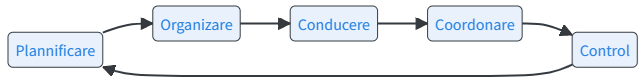
\includegraphics{images/functii_management.png}

}

\caption{Functiile Managementului}

\end{figure}%

Datele joacă un rol esențial în susținerea tuturor funcțiilor
managementului, contribuind la luarea deciziilor mai bine fundamentate
și la optimizarea performanței organizaționale. Să analizăm cum sunt
datele integrate în fiecare dintre aceste funcții:

\emph{1. Planificarea}\\
Planificarea este prima și cea mai importantă funcție a managementului,
deoarece stabilește obiectivele și strategia pentru atingerea acestora.
Analiza datelor este esențială în acest proces, oferind informații
precise care permit decidenților să:

\begin{itemize}
\tightlist
\item
  Proiecteze scenarii și previziuni: Utilizarea datelor istorice și a
  prognozelor statistice permite managerilor să anticipeze tendințele
  viitoare, riscurile și oportunitățile.\\
\item
  Stabilească obiective măsurabile: Datele oferă o bază concretă pentru
  setarea unor obiective clare și realiste, care pot fi monitorizate și
  ajustate în timp.\\
\item
  Evalueze resursele disponibile: Datele financiare și operaționale
  ajută managerii să înțeleagă mai bine ce resurse (umane, financiare,
  materiale) sunt disponibile și cum pot fi acestea utilizate mai
  eficient.
\end{itemize}

Exemplu practic: O companie de retail dorește să își extindă rețeaua de
magazine în alte regiuni. Managerii colectează date despre
comportamentul consumatorilor, venituri medii pe cap de locuitor, și
tendințele pieței din mai multe regiuni. Prin analizarea datelor
disponibile, aceștia pot:

\begin{itemize}
\tightlist
\item
  Identifica cele mai promițătoare regiuni: Pe baza datelor, se poate
  stabili unde există cerere ridicată pentru produsele oferite de
  companie.\\
\item
  Proiecta venituri viitoare: Utilizând modele predictive, managerii pot
  estima veniturile potențiale pentru fiecare regiune.\\
\item
  Planifica alocarea resurselor: Datele financiare și de resurse umane
  ajută la determinarea costurilor necesare pentru extindere și la
  alocarea eficientă a bugetului.
\end{itemize}

\emph{2. Organizarea}\\
Funcția de organizare se referă la structurarea resurselor și
activităților pentru a atinge obiectivele organizaționale. Datele sunt
esențiale pentru:

\begin{itemize}
\item
  Alocarea resurselor: Analiza datelor privind performanțele
  departamentelor sau echipelor permite managerilor să aloce resursele
  în mod eficient, acolo unde sunt cele mai necesare.
\item
  Structurarea proceselor: Datele despre fluxurile de lucru și
  activitățile operaționale pot dezvălui zonele ineficiente, permițând
  optimizarea proceselor și îmbunătățirea productivității.
\item
  Definirea responsabilităților: Analiza performanței individuale și
  colective, pe baza datelor, ajută la o mai bună definire a sarcinilor
  și responsabilităților în cadrul echipelor.
\end{itemize}

Exemplu practic: O instituție publică dorește să eficientizeze procesul
de alocare a resurselor pentru un proiect de infrastructură. Analiza
datelor istorice despre termenele de livrare și costurile diferitelor
furnizori le permite managerilor să:

\begin{itemize}
\tightlist
\item
  Selecteze cei mai buni furnizori: Pe baza datelor privind performanța
  furnizorilor anteriori (calitatea, costurile și punctualitatea),
  managerii pot lua decizii informate pentru contractarea serviciilor.\\
\item
  Optimizeze distribuția resurselor: Datele despre utilizarea anterioară
  a resurselor (materiale, echipamente) ajută la organizarea stocurilor
  și evitarea supraproducției sau a blocajelor de aprovizionare.\\
\item
  Definirea responsabilităților: Analiza datelor de performanță ale
  echipelor ajută la repartizarea sarcinilor în funcție de abilitățile
  și istoricul fiecărui membru al echipei.
\end{itemize}

\emph{3. Conducerea}\\
Funcția de conducere (leadership) presupune motivarea și ghidarea
echipei către atingerea obiectivelor organizaționale. Datele sprijină
această funcție prin:

\begin{itemize}
\item
  Monitorizarea performanței: Managerii pot utiliza datele pentru a
  urmări performanțele angajaților și pentru a oferi feedback în timp
  real, ajutând la menținerea moralului și motivației.
\item
  Stabilirea de obiective clare pentru echipă: Utilizarea datelor pentru
  a stabili obiective individuale și de echipă care sunt realiste și
  măsurabile.
\item
  Dezvoltarea abilităților: Datele referitoare la nevoile de formare și
  dezvoltare profesională permit managerilor să identifice domeniile în
  care echipa lor ar putea beneficia de instruire suplimentară.
\end{itemize}

Exemplu practic: Un manager de echipă dintr-o companie de IT dorește să
îmbunătățească performanța echipei. El analizează datele privind
productivitatea fiecărui membru al echipei și feedbackul de la
evaluările periodice. În baza acestor date:

\begin{itemize}
\tightlist
\item
  Stabilește obiective personalizate: Managerul setează obiective clare
  pentru fiecare membru al echipei în funcție de competențele și
  performanțele anterioare.\\
\item
  Oferă feedback continuu: Folosind date de performanță în timp real,
  managerul oferă feedback regulat și ajută echipa să se concentreze pe
  punctele forte și să îmbunătățească punctele slabe.\\
\item
  Motivarea echipei: Managerul folosește datele pentru a identifica
  momentele în care angajații au nevoie de sprijin suplimentar sau de
  recunoaștere pentru munca bine făcută, crescând astfel moralul
  echipei.
\end{itemize}

\emph{4. Coordonarea}\\
Coordonarea implică integrarea activităților și resurselor pentru a
atinge obiectivele în mod coerent și eficient. Datele permit o
coordonare eficientă prin:

\begin{itemize}
\tightlist
\item
  Sincronizarea activităților: Analiza datelor despre calendarul
  proiectelor și resursele disponibile ajută managerii să coordoneze
  eforturile echipelor și departamentelor, evitând blocajele.\\
\item
  Fluxuri de informații: Datele sunt esențiale pentru a asigura un flux
  continuu de informații între departamente și echipe, reducând astfel
  riscul de erori și întârzieri.\\
\item
  Gestionarea resurselor în timp real: Instrumentele de analiză a
  datelor permit managerilor să vadă în timp real starea resurselor și
  să facă ajustări rapide pentru a menține echilibrul în activități.
\end{itemize}

Exemplu practic: O fabrică de producție utilizează analiza datelor
pentru a coordona mai eficient fluxurile de producție între
departamente. Prin colectarea și analizarea datelor despre stocurile de
materii prime, capacitatea de producție și cerințele de livrare,
managerii:

\begin{itemize}
\tightlist
\item
  Asigură sincronizarea proceselor: Datele în timp real despre stocuri
  și termene de producție permit echipelor să își ajusteze fluxurile de
  lucru pentru a evita întârzierile sau stocurile prea mari.\\
\item
  Reduce riscul de blocaje: Managerii pot identifica în avans problemele
  potențiale de aprovizionare sau întârzierile în producție și pot
  coordona acțiunile pentru a preveni blocajele.\\
\item
  Gestionarea resurselor eficient: Datele privind productivitatea
  fiecărui departament ajută managerii să aloce resursele (timp,
  materiale, personal) în funcție de nevoile reale.
\end{itemize}

\emph{5. Controlul}\\
Funcția de control este esențială pentru a monitoriza progresul și a
asigura că organizația atinge obiectivele stabilite. Analiza datelor
joacă un rol crucial în:

\begin{itemize}
\tightlist
\item
  Evaluarea performanței: Datele sunt utilizate pentru a măsura
  performanțele în raport cu obiectivele stabilite. Analizele periodice
  permit managerilor să vadă unde sunt deviații și să intervină pentru a
  corecta cursul.\\
\item
  Corectarea deviațiilor: Datele oferă o imagine clară asupra abaterilor
  de la planul inițial, permițând managerilor să implementeze măsuri
  corective pentru a readuce organizația pe drumul cel bun.\\
\item
  Raportarea performanței: Utilizarea datelor pentru a genera rapoarte
  detaliate și tablouri de bord ajută la monitorizarea continuă a
  performanțelor și la identificarea problemelor înainte ca acestea să
  devină critice.
\end{itemize}

Exemplu practic: Un manager dintr-o companie de servicii financiare
utilizează datele de performanță ale angajaților și indicatorii
financiari pentru a evalua eficiența unui program recent implementat.
Folosind dashboard-uri PowerBI, managerul:

\begin{itemize}
\tightlist
\item
  Monitorizează în timp real obiectivele: Dashboard-urile permit
  urmărirea progresului către obiectivele financiare și operaționale
  stabilite.\\
\item
  Identifică deviațiile: Managerul poate observa rapid când o echipă sau
  un departament nu îndeplinește obiectivele stabilite și poate
  interveni pentru a oferi suport sau pentru a ajusta strategia.\\
\item
  Propune măsuri corective: Pe baza analizelor de date, managerul poate
  ajusta bugetul, aloca resurse suplimentare sau redefini procesele
  pentru a readuce proiectul pe calea cea bună.
\end{itemize}

În această secțiune am văzut cum datele sunt un element central pentru
îndeplinirea tuturor funcțiilor managementului, oferind suport pentru
decizii bine informate și pentru optimizarea proceselor în organizații.
Fie că este vorba despre planificarea pe termen lung sau evaluarea
performanței zilnice, datele oferă managerilor o imagine obiectivă și
clară asupra realității organizaționale.

\textbf{De ce este analiza datelor esențială pentru luarea deciziilor?}

Decizii bazate pe fapte și dovezi: În loc de a lua decizii pe baza
instinctelor sau a intuiției, organizațiile moderne se bazează din ce în
ce mai mult pe date pentru a ghida acțiunile și strategiile lor. Analiza
datelor oferă o bază factuală solidă pentru luarea deciziilor, reducând
riscurile asociate cu incertitudinea și lipsa de informații.

Identificarea tendințelor și tiparelor: Analiza datelor ajută la
identificarea tendințelor emergente, a modelelor de comportament sau a
anomaliilor care pot semnala oportunități sau riscuri. De exemplu, în
sectorul financiar, analiza datelor poate dezvălui tendințe ale pieței
sau poate identifica riscuri financiare iminente.

Optimizarea resurselor: Prin examinarea detaliată a datelor,
organizațiile pot identifica zonele în care resursele sunt utilizate
ineficient și pot ajusta procesele pentru a îmbunătăți eficiența și a
reduce costurile. Acest lucru este valabil atât pentru instituțiile
publice, care trebuie să gestioneze bugete limitate, cât și pentru
companiile private care doresc să maximizeze profiturile.

Monitorizarea performanței: Analiza datelor permite organizațiilor să
monitorizeze și să evalueze performanța programelor și inițiativelor în
timp real, permițând ajustări rapide atunci când este necesar. Acest
lucru este esențial în contextul economico-financiar, unde piețele și
condițiile economice se pot schimba rapid.

Susținerea inovației: Prin explorarea datelor, organizațiile pot
descoperi noi oportunități de creștere și inovație, fie că este vorba de
dezvoltarea unor produse noi, fie de optimizarea operațiunilor
existente.

În esență, analiza datelor nu doar că ajută la înțelegerea mai profundă
a situațiilor curente, dar permite și previzionarea evoluțiilor
viitoare, oferind decidenților informații esențiale pentru a naviga
provocările economice și financiare.

\section{Identificarea seturilor de date
relevante}\label{identificarea-seturilor-de-date-relevante}

Identificarea seturilor de date relevante este un pas esențial în
procesul de analiză a datelor, deoarece calitatea și relevanța
informațiilor folosite pot influența direct acuratețea concluziilor și
eficiența deciziilor luate. Fie că vorbim despre sectorul public sau
privat, este esențial ca analiza datelor să se bazeze pe informații
corecte, complete și relevante pentru obiectivele definite.

\textbf{Posibile etape în identificarea seturilor de date relevante}

\begin{enumerate}
\def\labelenumi{\arabic{enumi}.}
\item
  \emph{Definirea obiectivelor analizei}. Înainte de a începe căutarea
  datelor, este crucial să fie definite clar obiectivele analizei, asa
  cum am aratat și într-o secțiune precedentă. La ce întrebări se
  dorește să se răspundă? Ce rezultate se așteaptă să fie obținute? De
  exemplu, în cazul unei instituții publice care analizează
  performanțele bugetare, datele financiare și de execuție bugetară vor
  fi de interes. Definirea clară a obiectivelor ajută la filtrarea și
  identificarea celor mai relevante seturi de date.
\item
  \emph{Determinarea surselor de date disponibile}. Odată ce obiectivele
  sunt stabilite, următorul pas este identificarea surselor potențiale
  de date. Aceste surse pot fi interne (de exemplu, baze de date
  organizaționale) sau externe (de exemplu, date guvernamentale,
  statistici publice, date de piață). Sursele comune de date includ:\\
\end{enumerate}

\begin{itemize}
\tightlist
\item
  Surse publice: Eurostat, Institutul Național de Statistică (INS),
  OCDE, Banca Mondială, UNData.\\
\item
  Surse private: Baze de date ale companiilor private, cum ar fi
  Bloomberg, Thomson Reuters, sau datele disponibile de la firme de
  consultanță.\\
\item
  Surse interne: Date colectate de către organizație, cum ar fi
  rapoartele financiare interne, datele despre performanțele
  operaționale sau bazele de date cu clienți.
\end{itemize}

\begin{enumerate}
\def\labelenumi{\arabic{enumi}.}
\setcounter{enumi}{2}
\tightlist
\item
  \emph{Evaluarea calității datelor}. Nu toate datele disponibile sunt
  de încredere sau relevante pentru analiza propusă. Este esențial să se
  evalueze calitatea datelor înainte de utilizarea acestora. Criteriile
  principale de evaluare includ:\\
\end{enumerate}

\begin{itemize}
\tightlist
\item
  Acuratețea: Datele trebuie să fie corecte și validate.\\
\item
  Actualitatea: Datele trebuie să fie actualizate și relevante pentru
  perioada de interes.\\
\item
  Completitudinea: Seturile de date nu trebuie să conțină informații
  lipsă sau incomplete, deoarece acest lucru poate afecta acuratețea
  analizei.\\
\item
  Consistența: Datele din surse diferite ar trebui să fie consistente și
  să urmeze aceleași reguli de structurare și format.
\end{itemize}

\begin{enumerate}
\def\labelenumi{\arabic{enumi}.}
\setcounter{enumi}{3}
\item
  \emph{Relevanța datelor pentru obiectivele analizei}. După evaluarea
  calității, este important să se asigure că datele colectate sunt
  relevante pentru întrebările la care se dorește răspuns. Aceasta
  înseamnă să se selecteze acele date care oferă informații utile pentru
  analiza în cauză. De exemplu, dacă obiectivul este analiza veniturilor
  într-o regiune, datele despre veniturile medii per locuitor și
  cheltuielile de consum vor fi esențiale.
\item
  \emph{Accesibilitatea și utilizarea datelor}. Seturile de date pot fi
  disponibile în diverse formate (CSV, XML, JSON etc.), iar accesul la
  acestea poate varia. Unele date pot fi liber accesibile (Open Data),
  în timp ce altele pot necesita acces special sau abonament (de
  exemplu, în cazul bazelor de date comerciale). Este esențial să se
  asigure că datele pot fi descărcate, prelucrate și integrate cu
  ușurință în software-ul de analiză folosit.
\item
  \emph{Asigurarea conformității cu reglementările privind protecția
  datelor}. În special când lucrăm cu date personale, este important să
  respectăm reglementările privind protecția datelor (de exemplu, GDPR
  în Uniunea Europeană). Acest lucru presupune verificarea că seturile
  de date respectă normele legale și etice privind colectarea și
  utilizarea informațiilor personale.
\end{enumerate}

\textbf{Exemple practice de identificare a seturilor de date relevante}

\begin{enumerate}
\def\labelenumi{\arabic{enumi}.}
\tightlist
\item
  \emph{Analiza economică într-o instituție publică}\\
  O administrație publică dorește să analizeze performanțele economice
  regionale pentru a stabili unde ar trebui să investească în
  infrastructură. Sursele de date relevante pot include:\\
\end{enumerate}

\begin{itemize}
\tightlist
\item
  Date de la Institutul Național de Statistică (INS) despre produsul
  intern brut (PIB) pe regiuni.\\
\item
  Informații de la Eurostat privind rata șomajului, venitul mediu pe cap
  de locuitor și nivelurile de investiții regionale.\\
\item
  Date din rapoartele bugetare locale pentru a evalua capacitatea de
  investiții în fiecare regiune.
\end{itemize}

\begin{enumerate}
\def\labelenumi{\arabic{enumi}.}
\setcounter{enumi}{1}
\tightlist
\item
  \emph{Analiza pieței pentru o companie privată}\\
  O companie de retail dorește să intre pe o piață nouă și are nevoie de
  date despre comportamentul consumatorilor și concurența în acea
  regiune. Sursele de date relevante pot include:\\
\end{enumerate}

\begin{itemize}
\tightlist
\item
  Date demografice și despre venitul pe cap de locuitor din bazele de
  date publice, cum ar fi OCDE sau UNData.\\
\item
  Date despre preferințele de consum și obiceiurile de cumpărare din
  surse private sau studiile de piață realizate de companii de
  cercetare.\\
\item
  Date din propriile sisteme de management al clienților (CRM) pentru a
  înțelege tiparele de achiziție ale clienților actuali.
\end{itemize}

\begin{enumerate}
\def\labelenumi{\arabic{enumi}.}
\setcounter{enumi}{2}
\tightlist
\item
  \emph{Monitorizarea performanței bugetare într-o instituție publică}\\
  O primărie dorește să își evalueze performanțele bugetare pentru a
  optimiza cheltuielile și veniturile. Seturile de date relevante
  includ:\\
\end{enumerate}

\begin{itemize}
\tightlist
\item
  Execuția bugetară anuală și trimestrială din propriile rapoarte
  financiare interne.\\
\item
  Date privind veniturile din taxe și impozite colectate de la
  serviciile de finanțe.\\
\item
  Date privind cheltuielile de capital și de funcționare pentru fiecare
  departament din primărie.
\end{itemize}

Datele colectate trebuie să fie de înaltă calitate, relevante pentru
obiectivele organizaționale și accesibile într-un format compatibil cu
software-urile de analiză utilizate. În plus, trebuie să se respecte
reglementările privind protecția datelor și să se folosească surse de
încredere.

\subsection{Surse de date publice și private, inclusiv Open
Data}\label{surse-de-date-publice-ux219i-private-inclusiv-open-data}

Datele utilizate în analiza economico-financiară pot proveni dintr-o
varietate de surse, fie publice, fie private. În ultimii ani, o sursă
importantă de date a devenit și Open Data, un concept care promovează
accesul liber și gratuit la informațiile colectate de instituțiile
publice. În acest subcapitol vom explora diferitele surse de date,
modalitățile de accesare a acestora, și exemple concrete de utilizare a
datelor publice, private și deschise (Open Data).

\textbf{Surse de date publice}\\
Sursele de date publice sunt furnizate de guverne, organizații
internaționale și instituții publice și sunt de obicei accesibile fără
costuri pentru utilizatori. Aceste date sunt esențiale pentru analiza
economico-financiară, fiind deseori utilizate în raportările oficiale și
studiile de cercetare.

Exemple de surse de date publice:

\begin{enumerate}
\def\labelenumi{\arabic{enumi}.}
\tightlist
\item
  Eurostat (Oficiul de Statistică al Uniunii Europene)\\
\end{enumerate}

\begin{itemize}
\tightlist
\item
  Eurostat oferă acces la o gamă largă de date statistice legate de
  economie, populație, comerț, muncă, mediu și multe altele din toate
  țările membre ale Uniunii Europene. Aceste date sunt esențiale pentru
  comparații internaționale și evaluări la nivel european.\\
\item
  Exemplu de utilizare: Datele Eurostat pot fi folosite pentru analiza
  produsului intern brut (PIB) al țărilor UE sau pentru a studia ratele
  șomajului în diferite regiuni europene.
\end{itemize}

\begin{enumerate}
\def\labelenumi{\arabic{enumi}.}
\setcounter{enumi}{1}
\tightlist
\item
  Institutul Național de Statistică (INS)\\
\end{enumerate}

\begin{itemize}
\tightlist
\item
  INS furnizează date statistice detaliate despre România, acoperind
  domenii precum economie, populație, mediu, educație și sănătate.
  Datele sunt disponibile gratuit prin intermediul platformei online a
  INS.\\
\item
  Exemplu de utilizare: O instituție publică poate utiliza datele INS
  pentru a analiza dinamica populației sau evoluția indicilor de prețuri
  în diverse regiuni din România.
\end{itemize}

\begin{enumerate}
\def\labelenumi{\arabic{enumi}.}
\setcounter{enumi}{2}
\tightlist
\item
  OECD (Organizația pentru Cooperare și Dezvoltare Economică)\\
\end{enumerate}

\begin{itemize}
\tightlist
\item
  OECD oferă acces la o vastă bază de date economice și sociale,
  inclusiv informații despre comerț internațional, investiții, educație
  și sănătate. Aceste date sunt extrem de utile pentru comparațiile
  internaționale și pentru înțelegerea tendințelor globale.\\
\item
  Exemplu de utilizare: Companiile pot folosi datele OECD pentru a
  analiza nivelurile de investiții străine directe (ISD) în diferite
  țări, ca parte a strategiei de expansiune globală.
\end{itemize}

\begin{enumerate}
\def\labelenumi{\arabic{enumi}.}
\setcounter{enumi}{3}
\tightlist
\item
  UN Data (United Nations Data)\\
\end{enumerate}

\begin{itemize}
\tightlist
\item
  UN Data oferă acces la date statistice globale furnizate de agențiile
  Națiunilor Unite. Aceste date acoperă o gamă largă de domenii, de la
  dezvoltare economică la sănătate și educație.\\
\item
  Exemplu de utilizare: Analiza dezvoltării durabile pe baza datelor
  oferite de UN Data, pentru a evalua progresul în atingerea
  obiectivelor de dezvoltare durabilă (SDG) în diverse regiuni.
\end{itemize}

\textbf{Surse de date private}

Sursele de date private sunt de obicei disponibile prin intermediul
companiilor care colectează și vând date, sau care oferă acces la bazele
lor de date pe bază de abonament. Aceste date sunt adesea utilizate
pentru analize specializate și pentru luarea deciziilor strategice în
mediul privat.

Exemple de surse de date private:

\begin{enumerate}
\def\labelenumi{\arabic{enumi}.}
\tightlist
\item
  Bloomberg
\end{enumerate}

\begin{itemize}
\tightlist
\item
  Bloomberg oferă date financiare în timp real despre piețele de
  capital, tranzacții comerciale și economie globală. Aceste date sunt
  folosite de bănci, firme de investiții și companii pentru a lua
  decizii financiare bine informate.\\
\item
  Exemplu de utilizare: O firmă de investiții poate utiliza datele
  Bloomberg pentru a analiza tendințele piețelor bursiere și a lua
  decizii de tranzacționare.
\end{itemize}

\begin{enumerate}
\def\labelenumi{\arabic{enumi}.}
\setcounter{enumi}{1}
\tightlist
\item
  Thomson Reuters
\end{enumerate}

\begin{itemize}
\tightlist
\item
  Thomson Reuters furnizează date financiare și economice din surse
  globale, fiind un lider în furnizarea de informații pentru piețele
  financiare. Companiile folosesc aceste date pentru a analiza
  performanțele piețelor și pentru a realiza previziuni economice.\\
\item
  Exemplu de utilizare: Analiza tendințelor pieței de obligațiuni și
  evaluarea riscurilor asociate cu investițiile în diferite regiuni.
\end{itemize}

\begin{enumerate}
\def\labelenumi{\arabic{enumi}.}
\setcounter{enumi}{2}
\tightlist
\item
  Companii de cercetare de piață (ex. Nielsen, GfK)
\end{enumerate}

\begin{itemize}
\tightlist
\item
  Aceste companii colectează și vând date despre comportamentele de
  consum, preferințele de piață și tendințele de cumpărare. Datele lor
  sunt folosite de companii pentru a înțelege mai bine preferințele
  clienților și pentru a ajusta strategiile de marketing.\\
\item
  Exemplu de utilizare: O companie de retail poate folosi datele de
  cercetare de piață de la Nielsen pentru a înțelege comportamentele de
  achiziție dintr-o anumită regiune și pentru a ajusta sortimentul de
  produse în funcție de aceste date.
\end{itemize}

\begin{enumerate}
\def\labelenumi{\arabic{enumi}.}
\setcounter{enumi}{3}
\tightlist
\item
  Baze de date specializate
\end{enumerate}

\begin{itemize}
\tightlist
\item
  Acestea includ surse care oferă date sectoriale sau foarte
  specializate, cum ar fi date despre energia globală (de la IHS Markit)
  sau despre agricultura globală (de la FAPRI). Aceste date sunt utile
  pentru analize foarte specifice din diverse industrii.
\end{itemize}

\textbf{Open Data}

Open Data reprezintă o inițiativă globală care promovează accesul liber
și deschis la datele colectate de instituțiile publice, pentru a
încuraja inovația și transparența. Aceste date sunt disponibile gratuit
și pot fi reutilizate, redistribuite și integrate în orice analiză,
fiind o resursă importantă atât pentru sectorul public, cât și pentru
cel privat.

Exemple de surse Open Data:

\begin{enumerate}
\def\labelenumi{\arabic{enumi}.}
\tightlist
\item
  Portalul european de date (European Data Portal)
\end{enumerate}

\begin{itemize}
\tightlist
\item
  Acesta oferă acces la un număr mare de seturi de date din întreaga
  Uniune Europeană, acoperind domenii precum transportul, energia,
  sănătatea și administrația publică. Seturile de date sunt actualizate
  constant și sunt accesibile gratuit.\\
\item
  Exemplu de utilizare: O companie care dorește să implementeze soluții
  de energie regenerabilă poate utiliza datele despre consumul de
  energie și resursele disponibile în diferite țări europene pentru a
  face analize comparative.
\end{itemize}

\begin{enumerate}
\def\labelenumi{\arabic{enumi}.}
\setcounter{enumi}{1}
\tightlist
\item
  Data.gov (SUA)
\end{enumerate}

\begin{itemize}
\tightlist
\item
  Acesta este portalul de date deschise al guvernului SUA și oferă acces
  la sute de mii de seturi de date din diverse domenii, de la educație
  și sănătate la siguranță publică și mediu.\\
\item
  Exemplu de utilizare: Un start-up poate utiliza datele de la Data.gov
  pentru a dezvolta aplicații care sprijină transparența guvernamentală
  sau pentru a crea noi soluții tehnologice bazate pe date publice.
\end{itemize}

\begin{enumerate}
\def\labelenumi{\arabic{enumi}.}
\setcounter{enumi}{2}
\tightlist
\item
  Portaluri locale de date deschise (ex. date.gov.ro)
\end{enumerate}

\begin{itemize}
\tightlist
\item
  Portalurile de date deschise la nivel local sau național oferă acces
  la seturi de date relevante pentru regiuni sau țări specifice. De
  exemplu, data.gov.ro oferă acces la datele publice din România.\\
\item
  Exemplu de utilizare: O primărie poate folosi datele publice deschise
  pentru a analiza distribuția geografică a locuințelor și pentru a
  decide unde să aloce fonduri pentru infrastructura locală.
\end{itemize}

\begin{enumerate}
\def\labelenumi{\arabic{enumi}.}
\setcounter{enumi}{3}
\tightlist
\item
  data.gov.ro (România)
\end{enumerate}

\begin{itemize}
\tightlist
\item
  Punct central de acces pentru seturile de date deschise livrate de
  autoritățile și instituțiile administrației publice, ajutând publicul
  să găsească, să descarce și să folosească informațiile generate și
  deținute de structurile administrative.
\end{itemize}

\subsection{Evaluarea calității și relevanței
datelor}\label{evaluarea-calitux103ux21bii-ux219i-relevanux21bei-datelor}

Evaluarea calității și relevanței datelor este un pas critic în procesul
de analiză a datelor economico-financiare. Datele de calitate scăzută
sau nerelevante pot duce la concluzii greșite și la decizii
nefundamentate. Prin urmare, este esențial să fie evaluate din
perspectiva acurateței, completitudinii, consistenței și actualității
lor înainte de a fi utilizate în orice analiză.

\textbf{Dimensiuni esențiale în evaluarea calității datelor}

\begin{enumerate}
\def\labelenumi{\arabic{enumi}.}
\tightlist
\item
  Acuratețea (Corectitudinea datelor)\\
  Acuratețea se referă la măsura în care datele reflectă realitatea în
  mod corect. Datele inexacte sau eronate pot distorsiona rezultatele
  analizei, conducând la decizii greșite. \emph{Exemplu}: Dacă un set de
  date economice privind rata șomajului conține erori sau discrepanțe,
  analiza ulterioară va reflecta o imagine falsă a pieței muncii, ducând
  la concluzii incorecte cu privire la politicile de ocupare a forței de
  muncă.
\end{enumerate}

Cum evaluăm acuratețea:

\begin{itemize}
\tightlist
\item
  Compararea datelor cu alte surse independente și de încredere.\\
\item
  Verificarea logicii interne a datelor pentru a identifica anomalii
  (ex: valori negative acolo unde nu ar trebui să fie).\\
\item
  Verificarea datelor colectate manual sau automatizate pentru a detecta
  eventuale erori de introducere.
\end{itemize}

\begin{enumerate}
\def\labelenumi{\arabic{enumi}.}
\setcounter{enumi}{1}
\tightlist
\item
  Completitudinea\\
  Completitudinea datelor se referă la prezența tuturor valorilor
  necesare pentru a realiza o analiză corectă. Seturile de date
  incomplete pot distorsiona rezultatele analizei, mai ales atunci când
  lipsesc valori esențiale sau variabile importante.\\
  \emph{Exemplu}: Dacă datele despre cheltuielile bugetare ale unei
  instituții publice lipsesc pentru o anumită perioadă de timp, este
  imposibil să se realizeze o analiză completă a performanței financiare
  pentru acea perioadă.
\end{enumerate}

Cum evaluăm completitudinea:

\begin{itemize}
\tightlist
\item
  Verificarea existenței valorilor lipsă sau ``missing data''.\\
\item
  Utilizarea tehnicilor de imputare a valorilor lipsă (ex: medii, valori
  mediane) dacă datele lipsesc într-o proporție mică.\\
\item
  Evaluarea impactului valorilor lipsă asupra obiectivelor analizei
  (dacă lipsa acestora poate afecta semnificativ rezultatele).
\end{itemize}

\begin{enumerate}
\def\labelenumi{\arabic{enumi}.}
\setcounter{enumi}{2}
\tightlist
\item
  Consistența (Coerența datelor) Consistența se referă la măsura în care
  datele sunt armonizate și respectă aceleași reguli și formate, mai
  ales atunci când provin din surse diferite. Inconsistențele în
  structura sau formatul datelor pot crea probleme atunci când seturile
  de date sunt combinate sau comparate.\\
  \emph{Exemplu}: Într-o analiză economică la nivel internațional,
  datele despre PIB pot fi raportate în monede diferite sau pe ani
  diferiți. Lipsa conversiei corecte poate duce la erori majore în
  interpretarea rezultatelor.
\end{enumerate}

Cum evaluăm consistența:

\begin{itemize}
\tightlist
\item
  Verificarea formatelor de date (ex: verificarea unităților de măsură
  -- mii, milioane, procente).
\item
  Asigurarea că valorile au aceeași granularitate temporală (ex: date
  anuale, trimestriale) și spațială (ex: la nivel de țară, regiune).\\
\item
  Verificarea metadatelor pentru a înțelege proveniența și metodele de
  colectare ale fiecărui set de date.
\end{itemize}

\begin{enumerate}
\def\labelenumi{\arabic{enumi}.}
\setcounter{enumi}{3}
\tightlist
\item
  Actualitatea (Timeliness)\\
  Actualitatea se referă la cât de recent au fost colectate și
  actualizate datele. În anumite cazuri, datele vechi pot fi irelevante,
  în special într-un mediu dinamic cum este economia globală sau
  sectorul financiar.\\
  \emph{Exemplu}: Într-o analiză a pieței imobiliare, utilizarea datelor
  vechi de 5 ani poate duce la concluzii eronate, deoarece prețurile și
  tendințele pieței s-au schimbat între timp.
\end{enumerate}

Cum evaluăm actualitatea:

\begin{itemize}
\tightlist
\item
  Verificarea datei ultimei actualizări a seturilor de date.\\
\item
  Asigurarea că datele utilizate corespund perioadei de timp relevante
  pentru analiza propusă.\\
\item
  Compararea periodică a datelor cu surse noi sau actualizate pentru a
  asigura relevanța și acuratețea acestora.
\end{itemize}

\begin{enumerate}
\def\labelenumi{\arabic{enumi}.}
\setcounter{enumi}{4}
\tightlist
\item
  Relevanța\\
  Relevanța datelor se referă la măsura în care datele sunt potrivite
  pentru a răspunde la întrebările sau obiectivele analizei. Chiar dacă
  un set de date este corect și complet, poate fi irelevant pentru
  analiza curentă dacă nu oferă informații utile pentru deciziile care
  trebuie luate.\\
  \emph{Exemplu}: Dacă scopul este analiza performanței financiare a
  unei companii, datele despre satisfacția clienților, deși valoroase în
  alt context, nu sunt relevante pentru această analiză specifică.
\end{enumerate}

Cum evaluăm relevanța:

\begin{itemize}
\tightlist
\item
  Verificarea dacă datele răspund direct întrebărilor de analiză.\\
\item
  Asigurarea că seturile de date includ variabilele și indicatorii
  specifici obiectivelor analizei.\\
\item
  Evitarea utilizării excesive de date care pot complica analiza fără a
  aduce valoare adăugată.
\end{itemize}

\textbf{Factori suplimentari în evaluarea calității datelor}

\begin{enumerate}
\def\labelenumi{\arabic{enumi}.}
\tightlist
\item
  \emph{Proveniența datelor (sursa datelor)}. Este esențial să se știe
  de unde provin datele și cum au fost colectate. Datele colectate din
  surse necredibile sau neautorizate pot compromite întreaga analiză.
  Sursele de date oficiale și bine cunoscute, precum instituțiile
  statistice naționale sau organizațiile internaționale, sunt de obicei
  preferabile.
\end{enumerate}

Cum evaluăm proveniența datelor:

\begin{itemize}
\tightlist
\item
  Verificarea reputației sursei care furnizează datele.\\
\item
  Evaluarea metodologiei de colectare a datelor.\\
\item
  Utilizarea metadatelor pentru a înțelege procesele de curățare și
  prelucrare aplicate datelor.
\end{itemize}

\begin{enumerate}
\def\labelenumi{\arabic{enumi}.}
\setcounter{enumi}{1}
\tightlist
\item
  \emph{Documentația și metadatele}. Un set de date de calitate ar
  trebui să fie însoțit de documentație și metadate care să explice
  modul în care datele au fost colectate, prelucrate și structurate.
  Fără metadate, este dificil să se înțeleagă contextul și limitările
  datelor.
\end{enumerate}

Cum evaluăm documentația și metadatele:

\begin{itemize}
\tightlist
\item
  Verificarea existenței unui fișier cu metadate care descrie
  variabilele, unitățile de măsură și metodele de colectare.\\
\item
  Asigurarea că documentația este clară și ușor de înțeles.\\
\item
  Analizarea oricăror limitări sau precauții menționate în documentație
  care ar putea afecta analiza.
\end{itemize}

\begin{enumerate}
\def\labelenumi{\arabic{enumi}.}
\setcounter{enumi}{2}
\tightlist
\item
  Transparența și verificabilitatea Datele trebuie să fie transparente,
  în sensul că pot fi verificate și validate de către alte părți
  interesate. Această caracteristică este importantă mai ales în
  contextul instituțiilor publice, care trebuie să demonstreze
  transparență și responsabilitate în utilizarea și interpretarea
  datelor.
\end{enumerate}

Cum evaluăm transparența:

\begin{itemize}
\tightlist
\item
  Verificarea posibilității de a reproduce analiza pe baza datelor
  disponibile.\\
\item
  Asigurarea că sursele de date pot fi accesate și validate de către
  terți.\\
\item
  Verificarea că datele sunt prezentate într-un format accesibil și fără
  ambiguități.
\end{itemize}

Evaluarea calității și relevanței datelor este un proces esențial pentru
a asigura că analiza datelor economico-financiare este corectă, completă
și utilă pentru luarea deciziilor. Un set de date de înaltă calitate
oferă un fundament solid pentru analize precise și informații valoroase.
Acest proces de evaluare nu trebuie să fie neglijat, indiferent dacă
datele provin din surse publice, private sau din Open Data.

\subsection{Utilizarea platformelor de
date}\label{utilizarea-platformelor-de-date}

• Modalități de acces, descărcare și integrare a datelor • Prezentarea
unor platforme comune: Eurostat, INS, UN data, OECD Data

\section{Concepte de bază legate de formatarea
datelor}\label{concepte-de-bazux103-legate-de-formatarea-datelor}

(formatul și tipurile de date)

\subsection{Tipuri de surse de date (primare și
secundare)}\label{tipuri-de-surse-de-date-primare-ux219i-secundare}

text

\subsection{Tipuri de fișiere (CSV, XML, JSON) și utilizarea
lor}\label{tipuri-de-fiux219iere-csv-xml-json-ux219i-utilizarea-lor}

text

\subsection{Importanța și utilizarea
metadatelor}\label{importanux21ba-ux219i-utilizarea-metadatelor}

text

\section{Instrumente avansate pentru prelucrarea și analiza
datelor}\label{instrumente-avansate-pentru-prelucrarea-ux219i-analiza-datelor}

text

\bookmarksetup{startatroot}

\chapter{Instrumente și platformelor pentru analiza datelor}\label{cap2}

\section{Utilizarea R}\label{utilizarea-r}

text

\section{Utilizarea Python}\label{utilizarea-python}

text

\section{Utilizarea Excel}\label{utilizarea-excel}

text

\section{Utilizarea Power BI}\label{utilizarea-power-bi}

text

\bookmarksetup{startatroot}

\chapter{Introducere în analiza statistică}\label{cap3}

\section{Concepte de bază privind analiza
statistică}\label{concepte-de-bazux103-privind-analiza-statisticux103}

text

\section{Mărimile relative}\label{mux103rimile-relative}

text

\section{Sistematizarea datelor}\label{sistematizarea-datelor}

text

\section{Indicatorii de nivel}\label{indicatorii-de-nivel}

\subsection{Aplicații}\label{aplicaux21bii}

\subsubsection{1. Media unei serii
simple}\label{media-unei-serii-simple}

Se cunosc date privind veniturile salariale lunare (în lei/lună) ale
celor 80 de angajați din firma M. Caracteristicile serie sunt prezentate
în tabelul următor și ne propunem realizarea acestei analize descriptive
prin cele 4 platforme software.

\begin{table}[]
\begin{tabular}{lcccccc}
                             & grupe de venit (lei) & $n_i$ & $h_i$ & $x_i$ & $x_i n_i$ & $N_i$\^ \\                              & 0 – 1000             & 6     & 300   & 850   & 5100      & 6       \\
interval                     & 1001 - 1300          & 24    & 300   & 1150  & 27600     & 30      \\
interval median              & 1301 - 1600          & 30    & 300   & 1450  & 43500     & 60      \\
interval quartila superioară & 1601 - 1900          & 12    & 300   & 1750  & 21000     & 72      \\
                             & 1901 - 2200          & 5     & 300   & 2050  & 10250     & 77      \\
                             & 2201 - $\inf$        & 3     & 300   & 2350  & 7050      & 80      \\
                             & total                & 80    & -     & -     & 114500    &         \\ \end{tabular}
\end{table}

Să se determine venitul salarial mediu lunar al angajaților firmei.

\paragraph{Rezolvare prin R}\label{rezolvare-prin-r}

\begin{Shaded}
\begin{Highlighting}[]
\CommentTok{\# incarcarea datelor "venit.csv"}
\NormalTok{venit }\OtherTok{\textless{}{-}} \FunctionTok{read.csv}\NormalTok{(}\StringTok{"date/venit.csv"}\NormalTok{, }\AttributeTok{head =}\NormalTok{ T)}
\CommentTok{\# o vizualizare succinta a datelor}
\FunctionTok{head}\NormalTok{(venit)}
\end{Highlighting}
\end{Shaded}

\begin{verbatim}
  venit
1  1660
2  1410
3  1550
4  1820
5  1320
6  1340
\end{verbatim}

\begin{Shaded}
\begin{Highlighting}[]
\CommentTok{\# explorarea prelimiară a datelor}
\FunctionTok{summary}\NormalTok{(venit)}
\end{Highlighting}
\end{Shaded}

\begin{verbatim}
     venit     
 Min.   : 750  
 1st Qu.:1260  
 Median :1395  
 Mean   :1451  
 3rd Qu.:1605  
 Max.   :2360  
\end{verbatim}

\begin{Shaded}
\begin{Highlighting}[]
\CommentTok{\# intervalul datelor}
\FunctionTok{range}\NormalTok{(venit}\SpecialCharTok{$}\NormalTok{venit)}
\end{Highlighting}
\end{Shaded}

\begin{verbatim}
[1]  750 2360
\end{verbatim}

\begin{Shaded}
\begin{Highlighting}[]
\CommentTok{\# calculul mediei seriei simple}
\FunctionTok{mean}\NormalTok{(venit}\SpecialCharTok{$}\NormalTok{venit)}
\end{Highlighting}
\end{Shaded}

\begin{verbatim}
[1] 1450.875
\end{verbatim}

Venitul salarial mediu lunar al celor 80 angajați ai firmei este de
1450.875 lei/lună.

\paragraph{Rezolvare prin Python}\label{rezolvare-prin-python}

\begin{Shaded}
\begin{Highlighting}[]
\CommentTok{\# importarea librariilor necesare}
\ImportTok{import}\NormalTok{ pandas }\ImportTok{as}\NormalTok{ pd}

\CommentTok{\# incarcarea datelor "venit.csv"}
\NormalTok{venit }\OperatorTok{=}\NormalTok{ pd.read\_csv(}\StringTok{"date/venit.csv"}\NormalTok{)}

\CommentTok{\# o vizualizare succinta a datelor}
\BuiltInTok{print}\NormalTok{(venit.head())}
\end{Highlighting}
\end{Shaded}

\begin{verbatim}
   venit
0   1660
1   1410
2   1550
3   1820
4   1320
\end{verbatim}

\begin{Shaded}
\begin{Highlighting}[]
\CommentTok{\# explorarea preliminara a datelor}
\BuiltInTok{print}\NormalTok{(venit.describe())}
\end{Highlighting}
\end{Shaded}

\begin{verbatim}
             venit
count    80.000000
mean   1450.875000
std     338.683952
min     750.000000
25%    1260.000000
50%    1395.000000
75%    1605.000000
max    2360.000000
\end{verbatim}

\begin{Shaded}
\begin{Highlighting}[]
\CommentTok{\# intervalul datelor}
\BuiltInTok{print}\NormalTok{(venit[}\StringTok{\textquotesingle{}venit\textquotesingle{}}\NormalTok{].}\BuiltInTok{min}\NormalTok{(), venit[}\StringTok{\textquotesingle{}venit\textquotesingle{}}\NormalTok{].}\BuiltInTok{max}\NormalTok{())}
\end{Highlighting}
\end{Shaded}

\begin{verbatim}
750 2360
\end{verbatim}

\begin{Shaded}
\begin{Highlighting}[]
\CommentTok{\# calculul mediei seriei simple}
\BuiltInTok{print}\NormalTok{(venit[}\StringTok{\textquotesingle{}venit\textquotesingle{}}\NormalTok{].mean())}
\end{Highlighting}
\end{Shaded}

\begin{verbatim}
1450.875
\end{verbatim}

\paragraph{Rezolvare prin Excel}\label{rezolvare-prin-excel}

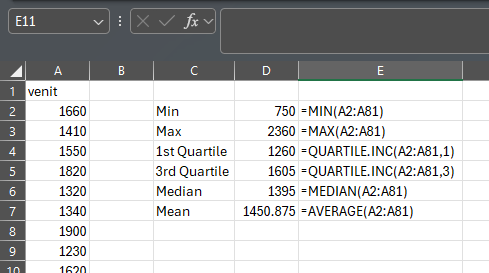
\includegraphics{date/medie_simpla.PNG}\\
\href{date/venit.xlsx}{venit.xlsx}

\paragraph{Rezolvare prin Power BI}\label{rezolvare-prin-power-bi}

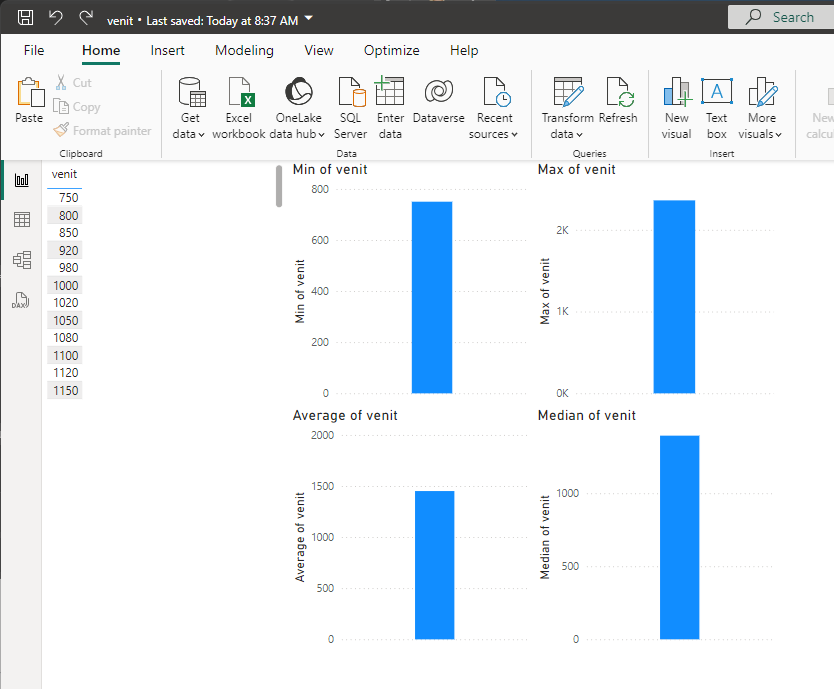
\includegraphics{date/medie_simpla_Pbi.png}

\subsubsection{2. Gruparea datelor - construirea seriilor de
distribuție}\label{gruparea-datelor---construirea-seriilor-de-distribuux21bie}

Exemplu: A fost efectuată o cercetare privind mărimea (măsurată pe baza
numărului de salariați) a 80 de firme industriale din orașul M. Datele
referitoare la numărul de salariați înregistrat în cursul observării
sunt următoarele:

\begin{table}[]
\begin{tabular}{|l|l|l|l|l|l|l|l|l|l|}
\hline
166 & 162 & 121 & 126 & 128 & 85  & 136 & 158 & 135 & 127 \\ \hline
141 & 142 & 92  & 148 & 177 & 80  & 156 & 188 & 205 & 144 \\ \hline
155 & 230 & 100 & 129 & 160 & 159 & 105 & 150 & 110 & 98  \\ \hline
182 & 102 & 128 & 198 & 115 & 122 & 124 & 163 & 130 & 133 \\ \hline
132 & 150 & 75  & 206 & 149 & 170 & 112 & 142 & 119 & 151 \\ \hline
134 & 224 & 135 & 236 & 126 & 175 & 215 & 130 & 121 & 128 \\ \hline
190 & 156 & 108 & 143 & 218 & 172 & 180 & 120 & 169 & 129 \\ \hline
123 & 156 & 142 & 127 & 133 & 146 & 139 & 140 & 138 & 138 \\ \hline
\end{tabular}
\end{table}

\paragraph{Rezolvare prin R}\label{rezolvare-prin-r-1}

\begin{Shaded}
\begin{Highlighting}[]
\CommentTok{\# incarcarea datele}
\NormalTok{grupare }\OtherTok{\textless{}{-}} \FunctionTok{read.csv}\NormalTok{(}\StringTok{"date/grupare.csv"}\NormalTok{, }\AttributeTok{head =}\NormalTok{ F)}
\FunctionTok{head}\NormalTok{(grupare)}
\end{Highlighting}
\end{Shaded}

\begin{verbatim}
   V1
1 166
2 162
3 121
4 126
5 128
6  85
\end{verbatim}

\begin{Shaded}
\begin{Highlighting}[]
\CommentTok{\# numarul de observatii}
\NormalTok{nobs }\OtherTok{\textless{}{-}} \FunctionTok{length}\NormalTok{(grupare}\SpecialCharTok{$}\NormalTok{V1)}
\NormalTok{nobs}
\end{Highlighting}
\end{Shaded}

\begin{verbatim}
[1] 80
\end{verbatim}

\begin{Shaded}
\begin{Highlighting}[]
\CommentTok{\# numărul de grupe}
\NormalTok{g }\OtherTok{\textless{}{-}} \FunctionTok{ceiling}\NormalTok{((}\DecValTok{2}\SpecialCharTok{*}\NormalTok{nobs)}\SpecialCharTok{\^{}}\NormalTok{(}\DecValTok{1}\SpecialCharTok{/}\DecValTok{3}\NormalTok{))}
\NormalTok{g}
\end{Highlighting}
\end{Shaded}

\begin{verbatim}
[1] 6
\end{verbatim}

\begin{Shaded}
\begin{Highlighting}[]
\CommentTok{\# valoarea maximă}
\NormalTok{xmax }\OtherTok{\textless{}{-}} \FunctionTok{max}\NormalTok{(grupare}\SpecialCharTok{$}\NormalTok{V1)}
\NormalTok{xmax}
\end{Highlighting}
\end{Shaded}

\begin{verbatim}
[1] 236
\end{verbatim}

\begin{Shaded}
\begin{Highlighting}[]
\CommentTok{\# valoarea minimă}
\NormalTok{xmin }\OtherTok{\textless{}{-}} \FunctionTok{min}\NormalTok{(grupare}\SpecialCharTok{$}\NormalTok{V1)}
\NormalTok{xmin}
\end{Highlighting}
\end{Shaded}

\begin{verbatim}
[1] 75
\end{verbatim}

\begin{Shaded}
\begin{Highlighting}[]
\CommentTok{\# determinarea înălțimii intervalelor}
\NormalTok{h }\OtherTok{\textless{}{-}}\NormalTok{ (xmax }\SpecialCharTok{{-}}\NormalTok{ xmin) }\SpecialCharTok{/}\NormalTok{ g}
\NormalTok{h}
\end{Highlighting}
\end{Shaded}

\begin{verbatim}
[1] 26.83333
\end{verbatim}

\begin{Shaded}
\begin{Highlighting}[]
\CommentTok{\# rotunjirea la o valoare superioară a intervalului}
\NormalTok{h }\OtherTok{\textless{}{-}} \FunctionTok{ceiling}\NormalTok{(h}\SpecialCharTok{/}\DecValTok{10}\NormalTok{) }\SpecialCharTok{*} \DecValTok{10}
\NormalTok{h}
\end{Highlighting}
\end{Shaded}

\begin{verbatim}
[1] 30
\end{verbatim}

\begin{Shaded}
\begin{Highlighting}[]
\CommentTok{\# limitele intervalelor de grupare}
\NormalTok{x1\_inf }\OtherTok{\textless{}{-}}\NormalTok{ xmin }\SpecialCharTok{{-}}\NormalTok{ (g}\SpecialCharTok{*}\NormalTok{h}\SpecialCharTok{{-}}\NormalTok{(xmax}\SpecialCharTok{{-}}\NormalTok{xmin))}\SpecialCharTok{/}\DecValTok{2}
\NormalTok{x1\_inf }
\end{Highlighting}
\end{Shaded}

\begin{verbatim}
[1] 65.5
\end{verbatim}

\begin{Shaded}
\begin{Highlighting}[]
\CommentTok{\# rotunjirea la o valoare superioară a limitei inferioare}
\NormalTok{x1\_inf }\OtherTok{\textless{}{-}} \FunctionTok{ceiling}\NormalTok{(x1\_inf}\SpecialCharTok{/}\DecValTok{10}\NormalTok{) }\SpecialCharTok{*} \DecValTok{10}
\NormalTok{x1\_inf}
\end{Highlighting}
\end{Shaded}

\begin{verbatim}
[1] 70
\end{verbatim}

\begin{Shaded}
\begin{Highlighting}[]
\CommentTok{\# dacă limita inferioară nu cuprinde valoarea minimă se reajustează limita inferioară}
\ControlFlowTok{if}\NormalTok{ (x1\_inf }\SpecialCharTok{\textgreater{}}\NormalTok{ xmin) \{x1\_inf }\OtherTok{\textless{}{-}}\NormalTok{ (}\FunctionTok{floor}\NormalTok{(x1\_inf}\SpecialCharTok{/}\DecValTok{10}\NormalTok{) }\SpecialCharTok{{-}} \DecValTok{1}\NormalTok{) }\SpecialCharTok{*} \DecValTok{10}\NormalTok{\}}

\CommentTok{\# determinarea intervalelor de frecvente}
\NormalTok{limite\_intervale }\OtherTok{\textless{}{-}} \FunctionTok{seq}\NormalTok{(}\AttributeTok{from =}\NormalTok{ x1\_inf, }\AttributeTok{to =} \DecValTok{250}\NormalTok{, }\AttributeTok{by =}\NormalTok{ h)}
\NormalTok{grupare}\SpecialCharTok{$}\NormalTok{interval }\OtherTok{\textless{}{-}} \FunctionTok{cut}\NormalTok{(grupare}\SpecialCharTok{$}\NormalTok{V1, }\AttributeTok{breaks =}\NormalTok{ limite\_intervale)}

\FunctionTok{library}\NormalTok{(dplyr)}
\end{Highlighting}
\end{Shaded}

\begin{verbatim}

Attaching package: 'dplyr'
\end{verbatim}

\begin{verbatim}
The following objects are masked from 'package:stats':

    filter, lag
\end{verbatim}

\begin{verbatim}
The following objects are masked from 'package:base':

    intersect, setdiff, setequal, union
\end{verbatim}

\begin{Shaded}
\begin{Highlighting}[]
\NormalTok{grupare }\SpecialCharTok{\%\textgreater{}\%} 
  \FunctionTok{group\_by}\NormalTok{(interval) }\SpecialCharTok{\%\textgreater{}\%}
  \FunctionTok{summarise}\NormalTok{(}\AttributeTok{frecvente =} \FunctionTok{n}\NormalTok{())}
\end{Highlighting}
\end{Shaded}

\begin{verbatim}
# A tibble: 6 x 2
  interval  frecvente
  <fct>         <int>
1 (70,100]          6
2 (100,130]        24
3 (130,160]        30
4 (160,190]        12
5 (190,220]         5
6 (220,250]         3
\end{verbatim}

\paragraph{Rezolvare prin Python}\label{rezolvare-prin-python-1}

\begin{Shaded}
\begin{Highlighting}[]
\ImportTok{import}\NormalTok{ pandas }\ImportTok{as}\NormalTok{ pd}
\ImportTok{import}\NormalTok{ numpy }\ImportTok{as}\NormalTok{ np}
\ImportTok{import}\NormalTok{ math}

\CommentTok{\# încărcarea datelor}
\NormalTok{grupare }\OperatorTok{=}\NormalTok{ pd.read\_csv(}\StringTok{"date/grupare.csv"}\NormalTok{, header}\OperatorTok{=}\VariableTok{None}\NormalTok{, names}\OperatorTok{=}\NormalTok{[}\StringTok{"V1"}\NormalTok{])}
\BuiltInTok{print}\NormalTok{(grupare.head())}
\end{Highlighting}
\end{Shaded}

\begin{verbatim}
    V1
0  166
1  162
2  121
3  126
4  128
\end{verbatim}

\begin{Shaded}
\begin{Highlighting}[]
\CommentTok{\# numărul de observații}
\NormalTok{nobs }\OperatorTok{=} \BuiltInTok{len}\NormalTok{(grupare[}\StringTok{"V1"}\NormalTok{])}
\BuiltInTok{print}\NormalTok{(nobs)}
\end{Highlighting}
\end{Shaded}

\begin{verbatim}
80
\end{verbatim}

\begin{Shaded}
\begin{Highlighting}[]
\CommentTok{\# numărul de grupe}
\NormalTok{g }\OperatorTok{=}\NormalTok{ math.ceil((}\DecValTok{2} \OperatorTok{*}\NormalTok{ nobs) }\OperatorTok{**}\NormalTok{ (}\DecValTok{1}\OperatorTok{/}\DecValTok{3}\NormalTok{))}
\BuiltInTok{print}\NormalTok{(g)}
\end{Highlighting}
\end{Shaded}

\begin{verbatim}
6
\end{verbatim}

\begin{Shaded}
\begin{Highlighting}[]
\CommentTok{\# valoarea maximă}
\NormalTok{xmax }\OperatorTok{=}\NormalTok{ grupare[}\StringTok{"V1"}\NormalTok{].}\BuiltInTok{max}\NormalTok{()}
\BuiltInTok{print}\NormalTok{(xmax)}
\end{Highlighting}
\end{Shaded}

\begin{verbatim}
236
\end{verbatim}

\begin{Shaded}
\begin{Highlighting}[]
\CommentTok{\# valoarea minimă}
\NormalTok{xmin }\OperatorTok{=}\NormalTok{ grupare[}\StringTok{"V1"}\NormalTok{].}\BuiltInTok{min}\NormalTok{()}
\BuiltInTok{print}\NormalTok{(xmin)}
\end{Highlighting}
\end{Shaded}

\begin{verbatim}
75
\end{verbatim}

\begin{Shaded}
\begin{Highlighting}[]
\CommentTok{\# determinarea înălțimii intervalelor}
\NormalTok{h }\OperatorTok{=}\NormalTok{ (xmax }\OperatorTok{{-}}\NormalTok{ xmin) }\OperatorTok{/}\NormalTok{ g}
\NormalTok{h }\OperatorTok{=}\NormalTok{ math.ceil(h }\OperatorTok{/} \DecValTok{10}\NormalTok{) }\OperatorTok{*} \DecValTok{10}  \CommentTok{\# rotunjire la cel mai apropiat multiplu de 10}
\BuiltInTok{print}\NormalTok{(h)}
\end{Highlighting}
\end{Shaded}

\begin{verbatim}
30
\end{verbatim}

\begin{Shaded}
\begin{Highlighting}[]
\CommentTok{\# limitele intervalelor de grupare}
\NormalTok{x1\_inf }\OperatorTok{=}\NormalTok{ xmin }\OperatorTok{{-}}\NormalTok{ (g }\OperatorTok{*}\NormalTok{ h }\OperatorTok{{-}}\NormalTok{ (xmax }\OperatorTok{{-}}\NormalTok{ xmin)) }\OperatorTok{/} \DecValTok{2}
\NormalTok{x1\_inf }\OperatorTok{=}\NormalTok{ math.ceil(x1\_inf }\OperatorTok{/} \DecValTok{10}\NormalTok{) }\OperatorTok{*} \DecValTok{10}  \CommentTok{\# rotunjire la cel mai apropiat multiplu de 10}

\CommentTok{\# ajustarea limitei inferioare dacă este necesar}
\ControlFlowTok{if}\NormalTok{ x1\_inf }\OperatorTok{\textgreater{}}\NormalTok{ xmin:}
\NormalTok{    x1\_inf }\OperatorTok{=}\NormalTok{ (math.floor(x1\_inf }\OperatorTok{/} \DecValTok{10}\NormalTok{) }\OperatorTok{{-}} \DecValTok{1}\NormalTok{) }\OperatorTok{*} \DecValTok{10}
\BuiltInTok{print}\NormalTok{(x1\_inf)}
\end{Highlighting}
\end{Shaded}

\begin{verbatim}
70
\end{verbatim}

\begin{Shaded}
\begin{Highlighting}[]
\CommentTok{\# determinarea intervalelor de frecvențe}
\NormalTok{limite\_intervale }\OperatorTok{=}\NormalTok{ np.arange(x1\_inf, }\DecValTok{250} \OperatorTok{+}\NormalTok{ h, h)}
\NormalTok{grupare[}\StringTok{\textquotesingle{}interval\textquotesingle{}}\NormalTok{] }\OperatorTok{=}\NormalTok{ pd.cut(grupare[}\StringTok{\textquotesingle{}V1\textquotesingle{}}\NormalTok{], bins}\OperatorTok{=}\NormalTok{limite\_intervale)}

\CommentTok{\# calculul frecvențelor pe intervale}
\NormalTok{frecvente }\OperatorTok{=}\NormalTok{ grupare.groupby(}\StringTok{\textquotesingle{}interval\textquotesingle{}}\NormalTok{).size().reset\_index(name}\OperatorTok{=}\StringTok{\textquotesingle{}frecvente\textquotesingle{}}\NormalTok{)}
\BuiltInTok{print}\NormalTok{(frecvente)}
\end{Highlighting}
\end{Shaded}

\begin{verbatim}
     interval  frecvente
0   (70, 100]          6
1  (100, 130]         24
2  (130, 160]         30
3  (160, 190]         12
4  (190, 220]          5
5  (220, 250]          3
\end{verbatim}

\paragraph{Rezolvare prin Excel}\label{rezolvare-prin-excel-1}

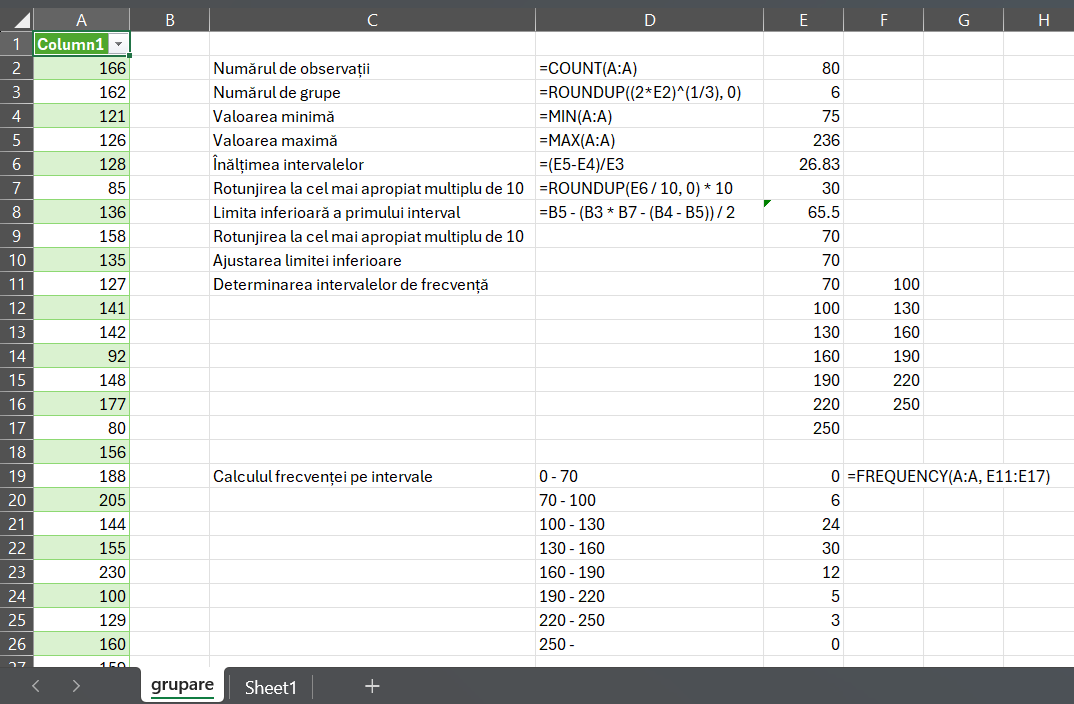
\includegraphics{date/grupare.PNG}
\href{date/grupare.xlsx}{grupare.xlsx}

\paragraph{Rezolvare prin Power BI}\label{rezolvare-prin-power-bi-1}

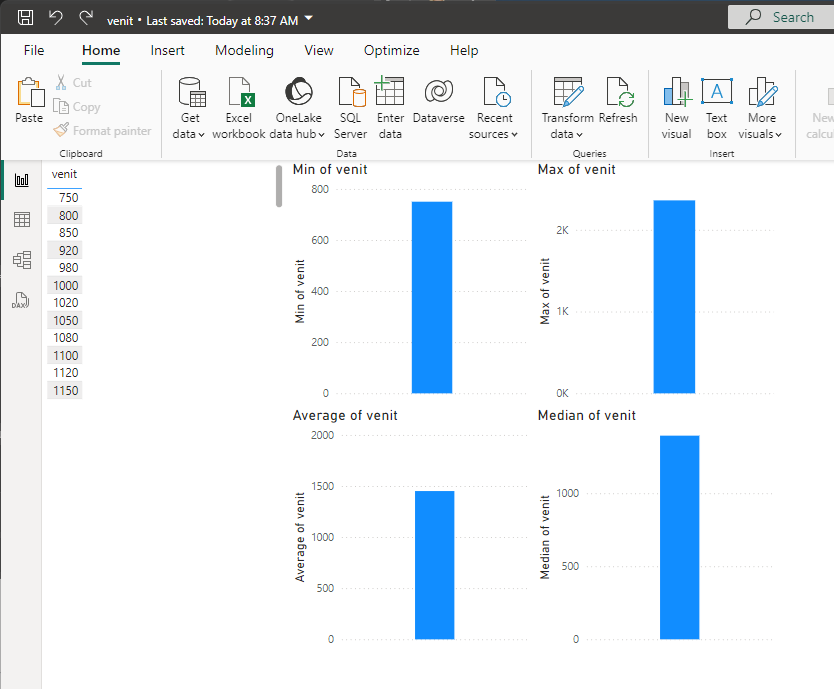
\includegraphics{date/medie_simpla_Pbi.png}

\section{Indicatorii variației}\label{indicatorii-variaux21biei}

• abateri, dispersie, abatere standard, repartiție, asimetrie,
concentrare

\section{Vizualizarea datelor}\label{vizualizarea-datelor}

text

\bookmarksetup{startatroot}

\chapter{Analiza datelor economico-financiare}\label{cap4}

\section{Indicatori economici și
financiari}\label{indicatori-economici-ux219i-financiari}

text

\section{Principii de bază în economie și finanțe
publice}\label{principii-de-bazux103-uxeen-economie-ux219i-finanux21be-publice}

text

\section{Analiza indicatorilor financiari ai instituțiilor
publice}\label{analiza-indicatorilor-financiari-ai-instituux21biilor-publice}

text

\bookmarksetup{startatroot}

\chapter{Analiza bugetară}\label{cap5}

\section{Structura bugetului public}\label{structura-bugetului-public}

text

\section{Metode de evaluare a performanței
bugetare}\label{metode-de-evaluare-a-performanux21bei-bugetare}

text

\section{Analiza deviațiilor și optimizarea
bugetară}\label{analiza-deviaux21biilor-ux219i-optimizarea-bugetarux103}

text

\bookmarksetup{startatroot}

\chapter{Analiza datelor sociale}\label{cap6}

\section{Introducere în analiza datelor
sociale}\label{introducere-uxeen-analiza-datelor-sociale}

\subsection{Definirea conceptului de date
sociale}\label{definirea-conceptului-de-date-sociale}

text

\subsection{Importanța datelor sociale în deciziile economice și
publice}\label{importanux21ba-datelor-sociale-uxeen-deciziile-economice-ux219i-publice}

text

\subsection{Rolul datelor sociale în cercetare și planificare
strategică}\label{rolul-datelor-sociale-uxeen-cercetare-ux219i-planificare-strategicux103}

text

\section{Tipuri de date sociale}\label{tipuri-de-date-sociale}

\subsection{Date demografice (vârstă, gen,
educație)}\label{date-demografice-vuxe2rstux103-gen-educaux21bie}

text

\subsection{Date privind ocuparea forței de muncă și
veniturile}\label{date-privind-ocuparea-forux21bei-de-muncux103-ux219i-veniturile}

text

\subsection{Date despre condițiile de trai (sănătate,
locuințe)}\label{date-despre-condiux21biile-de-trai-sux103nux103tate-locuinux21be}

text

\subsection{Date privind comportamentele sociale și
culturale}\label{date-privind-comportamentele-sociale-ux219i-culturale}

text

\subsection{Metode de colectare (sondaje, recensăminte, date
administrative)}\label{metode-de-colectare-sondaje-recensux103minte-date-administrative}

text

\section{Indicatori sociali}\label{indicatori-sociali}

\subsection{Indicatori demografici (rata natalității, mortalității,
migrației)}\label{indicatori-demografici-rata-natalitux103ux21bii-mortalitux103ux21bii-migraux21biei}

text

\subsection{Indicatori de sărăcie și incluziune
socială}\label{indicatori-de-sux103rux103cie-ux219i-incluziune-socialux103}

text

\subsection{Indicatori privind educația și
sănătatea}\label{indicatori-privind-educaux21bia-ux219i-sux103nux103tatea}

text

\subsection{Indicatori ai ocupării și
veniturilor}\label{indicatori-ai-ocupux103rii-ux219i-veniturilor}

text

\section{Analiza statistică a datelor
sociale}\label{analiza-statisticux103-a-datelor-sociale}

\subsection{Metode descriptive (medii, distribuții,
dispersie)}\label{metode-descriptive-medii-distribuux21bii-dispersie}

text

\subsection{Corelații între variabile
sociale}\label{corelaux21bii-uxeentre-variabile-sociale}

text

\subsection{Limitările și capcanele interpretării datelor
sociale}\label{limitux103rile-ux219i-capcanele-interpretux103rii-datelor-sociale}

text

\section{Aplicații practice în analiza datelor
sociale}\label{aplicaux21bii-practice-uxeen-analiza-datelor-sociale}

\subsection{Analiza inegalităților sociale și
economice}\label{analiza-inegalitux103ux21bilor-sociale-ux219i-economice}

text

\subsection{Evaluarea impactului politicilor publice asupra grupurilor
vulnerabile}\label{evaluarea-impactului-politicilor-publice-asupra-grupurilor-vulnerabile}

text

\subsection{Studiul fenomenelor demografice și impactul asupra pieței
muncii}\label{studiul-fenomenelor-demografice-ux219i-impactul-asupra-pieux21bei-muncii}

text

\subsection{Exemple de studii de caz bazate pe date
sociale}\label{exemple-de-studii-de-caz-bazate-pe-date-sociale}

text

\bookmarksetup{startatroot}

\chapter{Etapele analizei datelor}\label{cap7}

• cu exemple practice în Excel, Power BI, R, Python

\section{Definirea obiectivelor
analizei}\label{definirea-obiectivelor-analizei}

text

\section{Colectarea datelor}\label{colectarea-datelor}

text

\section{Importarea datelor}\label{importarea-datelor}

text

\section{Stocarea datelor}\label{stocarea-datelor}

text

\section{Curățarea datelor}\label{curux103ux21barea-datelor}

• Tratarea duplicatelor, gestionarea valorilor lipsă

\section{Agregarea datelor}\label{agregarea-datelor}

• Filtrarea/selectarea și agregarea datelor

\section{Analiza descriptivă a seturilor de
date}\label{analiza-descriptivux103-a-seturilor-de-date}

• Tabele de frecvență, diagrame de distribuție • Analiza distribuțiilor
și identificarea valorile anormale (outliers)

\section{Interpretarea rezultatelor}\label{interpretarea-rezultatelor}

text

\section{Vizualizarea rezultatelor}\label{vizualizarea-rezultatelor}

text

\section{Diseminarea rezultatelor
analizei}\label{diseminarea-rezultatelor-analizei}

text

\bookmarksetup{startatroot}

\chapter{Crearea și partajarea rapoartelor și tablourilor de
bord}\label{cap8}

\section{Crearea rapoartelor și tablourilor de
bord}\label{crearea-rapoartelor-ux219i-tablourilor-de-bord}

\subsection{Dezvoltarea de rapoarte interactive și tablouri de bord în
Power
BI.}\label{dezvoltarea-de-rapoarte-interactive-ux219i-tablouri-de-bord-uxeen-power-bi.}

text

\subsection{Utilizarea storytelling-ului în prezentarea
datelor.}\label{utilizarea-storytelling-ului-uxeen-prezentarea-datelor.}

text

\section{Partajarea și colaborarea pe
rapoarte}\label{partajarea-ux219i-colaborarea-pe-rapoarte}

\subsection{Tehnici de partajare a rapoartelor și tablourilor de bord în
organizație}\label{tehnici-de-partajare-a-rapoartelor-ux219i-tablourilor-de-bord-uxeen-organizaux21bie}

text

\subsection{Utilizarea platformelor de colaborare (e.g., Google Drive,
SharePoint)}\label{utilizarea-platformelor-de-colaborare-e.g.-google-drive-sharepoint}

text

\bookmarksetup{startatroot}

\chapter{Calitatea datelor}\label{cap9}

\section{Standarde, ghiduri și
monitorizare}\label{standarde-ghiduri-ux219i-monitorizare}

text

\section{Metodologii}\label{metodologii}

text

\section{Metadate}\label{metadate}

text

\section{Clasificări și
nomenclatoare}\label{clasificux103ri-ux219i-nomenclatoare}

\subsection{ceva}\label{ceva}

text

\section{Rapoarte de calitate}\label{rapoarte-de-calitate}

text

\section{Etica și transparența}\label{etica-ux219i-transparenux21ba}

text

\bookmarksetup{startatroot}

\chapter*{Bibliografie}\label{bibliografie}
\addcontentsline{toc}{chapter}{Bibliografie}

\markboth{Bibliografie}{Bibliografie}

Bibliografie

\phantomsection\label{refs}
\begin{CSLReferences}{1}{0}
\bibitem[\citeproctext]{ref-caragea2015}
Caragea, Nicoleta. 2015. \emph{\href{}{Statistică - Concepte Și Metode
de Analiză a Datelor}}. 1st ed. București, România: Editura MUSTANG.

\bibitem[\citeproctext]{ref-dusa2015}
Dușa, Adrian, Nicoleta Caragea, and Ciprian Alexandru. 2015. \emph{{R}
Cu Aplicații În Statistică}. 1st ed. București, România: Editura
Universității București.
\url{https://editura-unibuc.ro/magazin/stiinte-socio-umane/r-cu-aplicatii-in-statistica/}.

\bibitem[\citeproctext]{ref-xie2015}
Xie, Yihui. 2015. \emph{Dynamic Documents with {R} and Knitr}. 2nd ed.
Boca Raton, Florida: Chapman; Hall/CRC. \url{http://yihui.name/knitr/}.

\end{CSLReferences}


\backmatter


\end{document}
